\documentclass{article}
\usepackage[backend=biber]{biblatex}
\usepackage[german]{babel}
\usepackage{graphicx}
\usepackage{enumitem}
\usepackage{listings}
\usepackage{float}
\graphicspath{ {./img/} }

\setlength{\parindent}{0pt}

\bibliography{ByzantinischeFehler}

\title{Byzantinische Fehler}
\author{Matthias Reumann}
\date{\today}

\begin{document}

\maketitle

\newpage

\tableofcontents

\newpage

\section{Byzantinische Fehler}

\subsection{Definition}

Byzantinische Fehler treten in verteilten Systemen auf, 
wenn fehlerhafte Nachrichten von einem Knoten versendet werden, 
die von der Struktur und vom Inhalt nicht von fehlerfreien
unterscheidet werden können. \cite{esraberlin} 

\medskip 

Den Namen hat diese Fehlerklasse im Jahr 1982 von Lamport et. al. im 
Papier \textit{The Byzantine Generals Problem} erhalten.\cite{generals}
In diesem werden Byzantinische Fehler durch das abstrakte Beispiel der Byzantinischen Generäle näher erklärt.

\subsection{Anwendungen}
Da Fehlentscheidungen katastrophale Folgen hätten, wird in Boeing Flugzeugsystemen 
Byzantinischen Fehlern eine hohe Bedeutung zugewiesen.
Das Raumfahrtunternehmen SpaceX beachtet byzantinische Fehler in ihren Dragon Raumschiffen, 
welche Astronauten zur ISS transportieren sollen. 
Um die Integrität der Blockchain zu gewährleisten, ist die Implementierung von Bitcoin 
Byzantinische Fehler Tolerant (BFT).

\section{Problem der byzantinischen Generäle}
\label{sec:generals}
Mehrere Generäle und ihre Truppen umzingeln eine feindliche Stadt. 
Da diese voneinander räumlich getrennt sind können sie nur über Boten miteinander kommunizieren.
Jeder General beobachtet den gemeinsamen Feind und schlussendlich muss
eine gemeinsame Entscheidung getroffen werden um den Feind zu besiegen. 
Jedoch könnten unter den Generälen Verräter sein, deren Ziel es ist eine gemeinsame Entscheidung 
der loyalen Generäle zu verhindern. 

\medskip 

Die Generäle müssen einen Algorithmus finden der garantiert, dass

\begin{enumerate}[label=(\alph*)]
\item Alle loyalen Generäle die gleiche Entscheidung treffen 
\item Eine geringe Anzahl an Verrätern die loyalen Generäle nicht zu einer Fehlentscheidung führt
\end{enumerate}

Eine Entscheidung unter den Generälen wird gefällt indem jeder General seine Informationen an die anderen Generäle weitergibt. 
Die Nachricht gesendet vom $i$.ten General wird als \textit{v(i)} bezeichnet.
Jeder General erhält die Nachrichten \textit{v(1)} bis \textit{v(n)}, wobei $n$ die Anzahl der Generäle darstellt. 

Die finale Entscheidung wird durch die absolute Mehrheit der Werte dieser Nachrichten
bestimmt. In diesem konkreten Beispiel können die Werte entweder \textit{ANGRIFF} oder \textit{RÜCKZUG} sein.

Allerdings könnte es sein, dass ein Verräter unterschiedliche Werte zu unterschiedlichen Generälen sendet, 
was widerum bedeutet, dass loyale Generäle unterschiedliche \textit{v(i)} Werte besitzen. 

\medskip 

Deshalb müssen sogennante \textit{interactive consistency conditions} gelten.
Ein führender General, auch Commander genannt, sendet einen Befehl an seine $n - 1$ Leutnant 
Generäle so, dass:

\smallskip 

\begin{tabular}{l l}
IC1 & Alle loyalen Lieutenants den gleichen Befehl ausführen \\
IC2 & Wenn der Commander loyal ist, dann befolgt jeder loyale Leutnant seinen Befehl
\end{tabular}

\subsection{Beispiel mit drei Generälen}
In diesem Abschnitt wird eine Situation beschrieben in der drei Generäle miteinander kommunzieren. 
Wichtig dabei ist, dass niemand der loyalen Generäle weiß wer der Verräter ist. 

\medskip

In Abbildung \ref{fig:general1} ist Lieutenant 2 (L2) der Verräter. Der loyale Commander
sendet den Befehl \textit{ANGRIFF} an beide Lieutenant L1 und L2. Zur Verifizierung sendet L2 L1 die Nachricht,
er habe den Befehl \textit{RÜCKZUG} erhalten. 
L1 hat nun die Nachrichten \textit{ANGRIFF} und \textit{RÜCKZUG} und 
kann auf Grund dessen keine eindeutige Entscheidung treffen. Eine mögliche Lösung wäre
immer die Entscheidung des Commanders zu übernehmen. 

\begin{figure}[H]
    \centering
    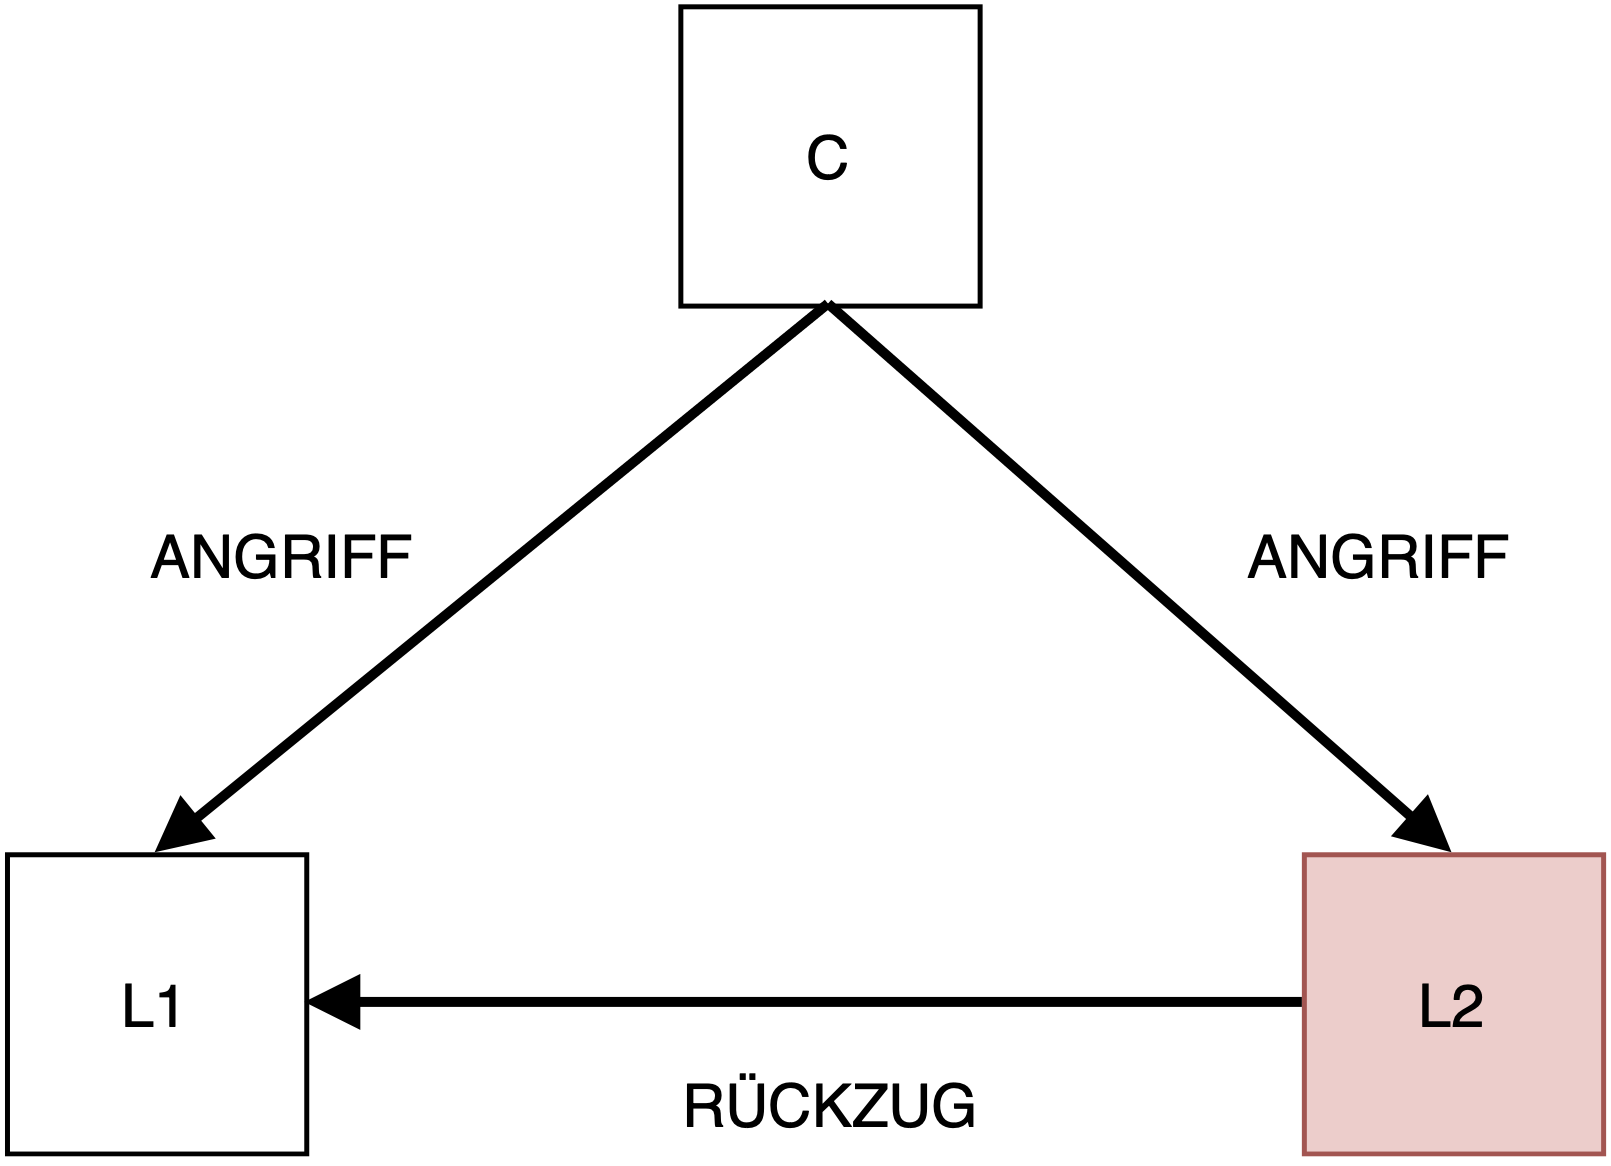
\includegraphics[width=0.7\textwidth]{general1.png}
    \caption{L2 ist der Verräter. L1 muss den Befehl des Commanders auführen um die IC2 einzuhalten.}
    \label{fig:general1}
\end{figure}

Im nächsten Szenario (Abbildung \ref{fig:general2}) ist der Commander der Verräter. Dieser sendet unterschiedliche 
Befehle an L1 und L2. Für L1 ist es die exakt selbe Situation 
wie in Abbildung \ref{fig:general1}. L2 steht vor dem selben Problem. 
Wird hier jedoch die gleiche Argumentation wie bei L1 angewandt, führen L1 und L2 verschiedene Befehle aus. 

\begin{figure}[H]
    \centering
    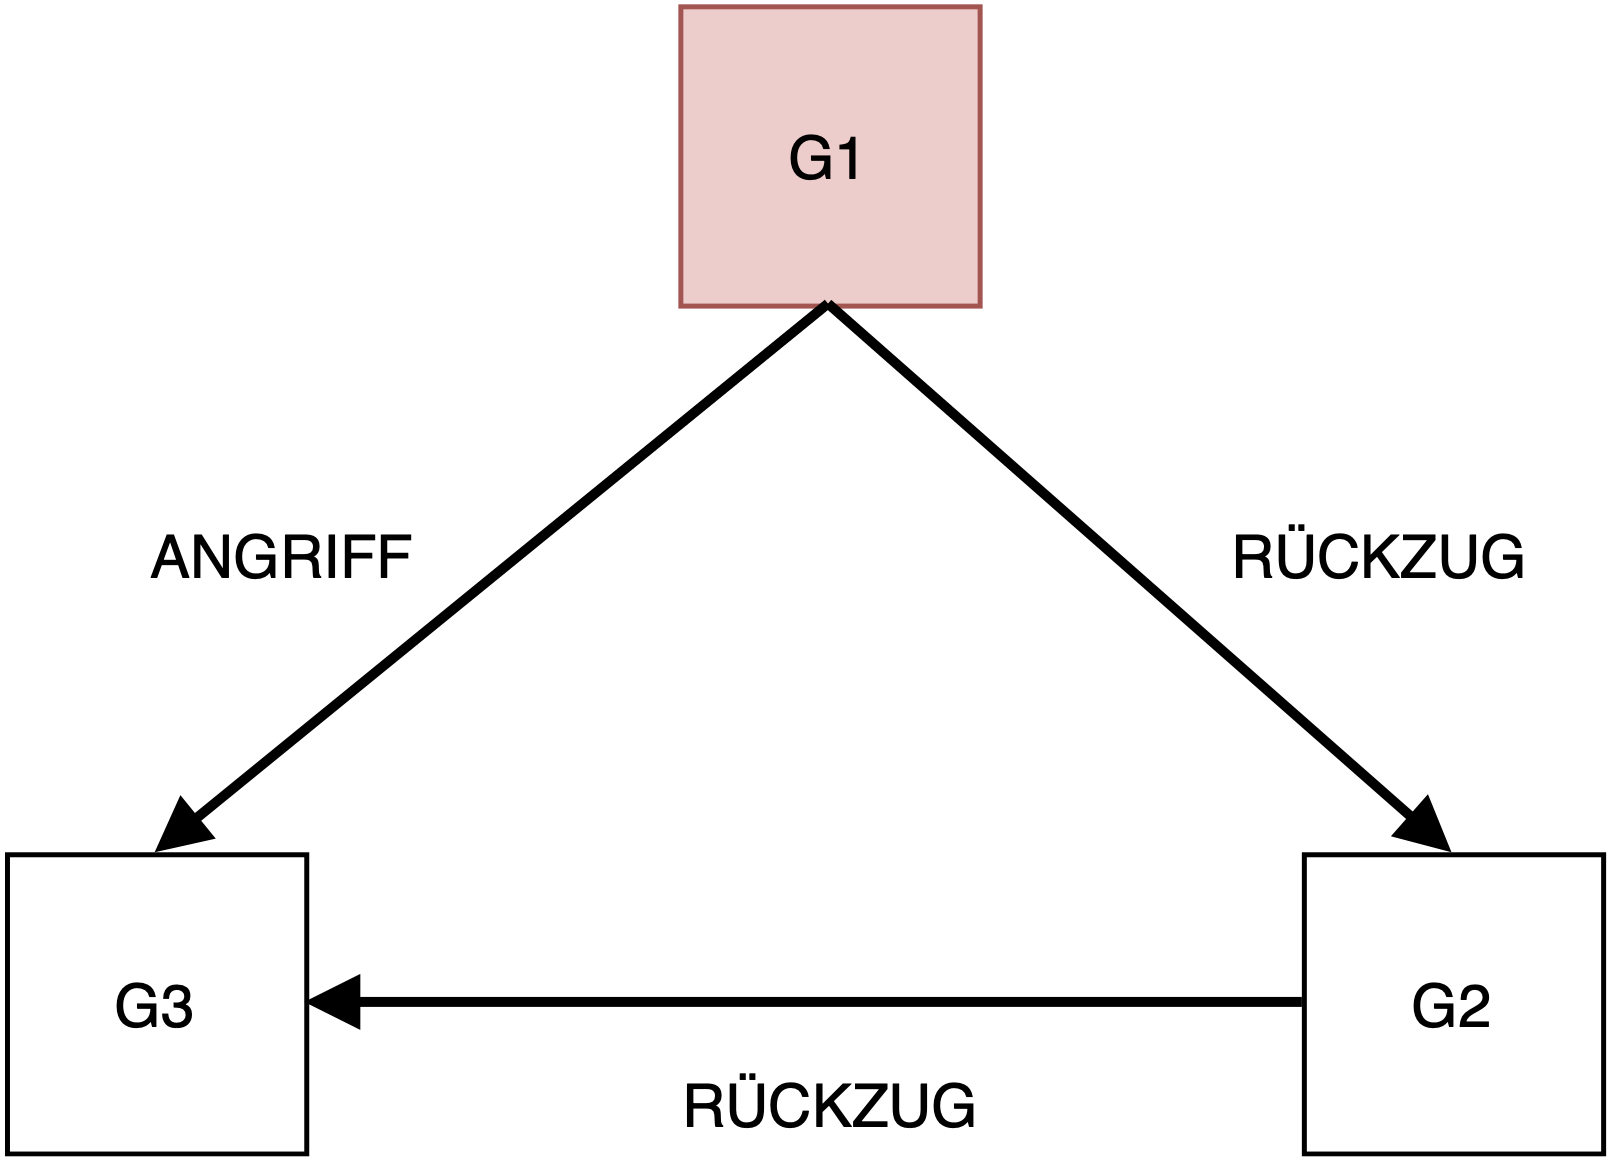
\includegraphics[width=0.7\textwidth]{general2.png}
    \caption{Der Commander ist der Verräter. Für L1 ist es die selbe Situtation wie in Abbildung \ref{fig:general1}.}
    \label{fig:general2}
\end{figure}

Wie aus diesem Beispiel hervorgeht, existiert keine Lösung für drei Generäle mit einem Verräter. 
Um einen byzantinischen Fehler zu erkennen muss daher folgende Eigenschaft gelten: $n \geq 3m + 1$, 
wobei $n$ die Anzahl der Generäle und $m$ die Anzahl der Verräter in diesem System ist. Mit anderen Worten, 
mehr als zwei Drittel müssen loyal sein, um einen byzantinischen Fehler zu erkennen. 

\subsection{Mögliche Lösungen}
Eine mögliche Lösung des Problems ist das Hinzufügen eines weiteren Generals. 
Dadurch kann, wenn jeder Leutnant seine erhaltene Nachricht an die anderen Leutnants 
sendet, genau ein byzantinischer Fehler erkannt werden. 

\begin{figure}[H]
    \centering
    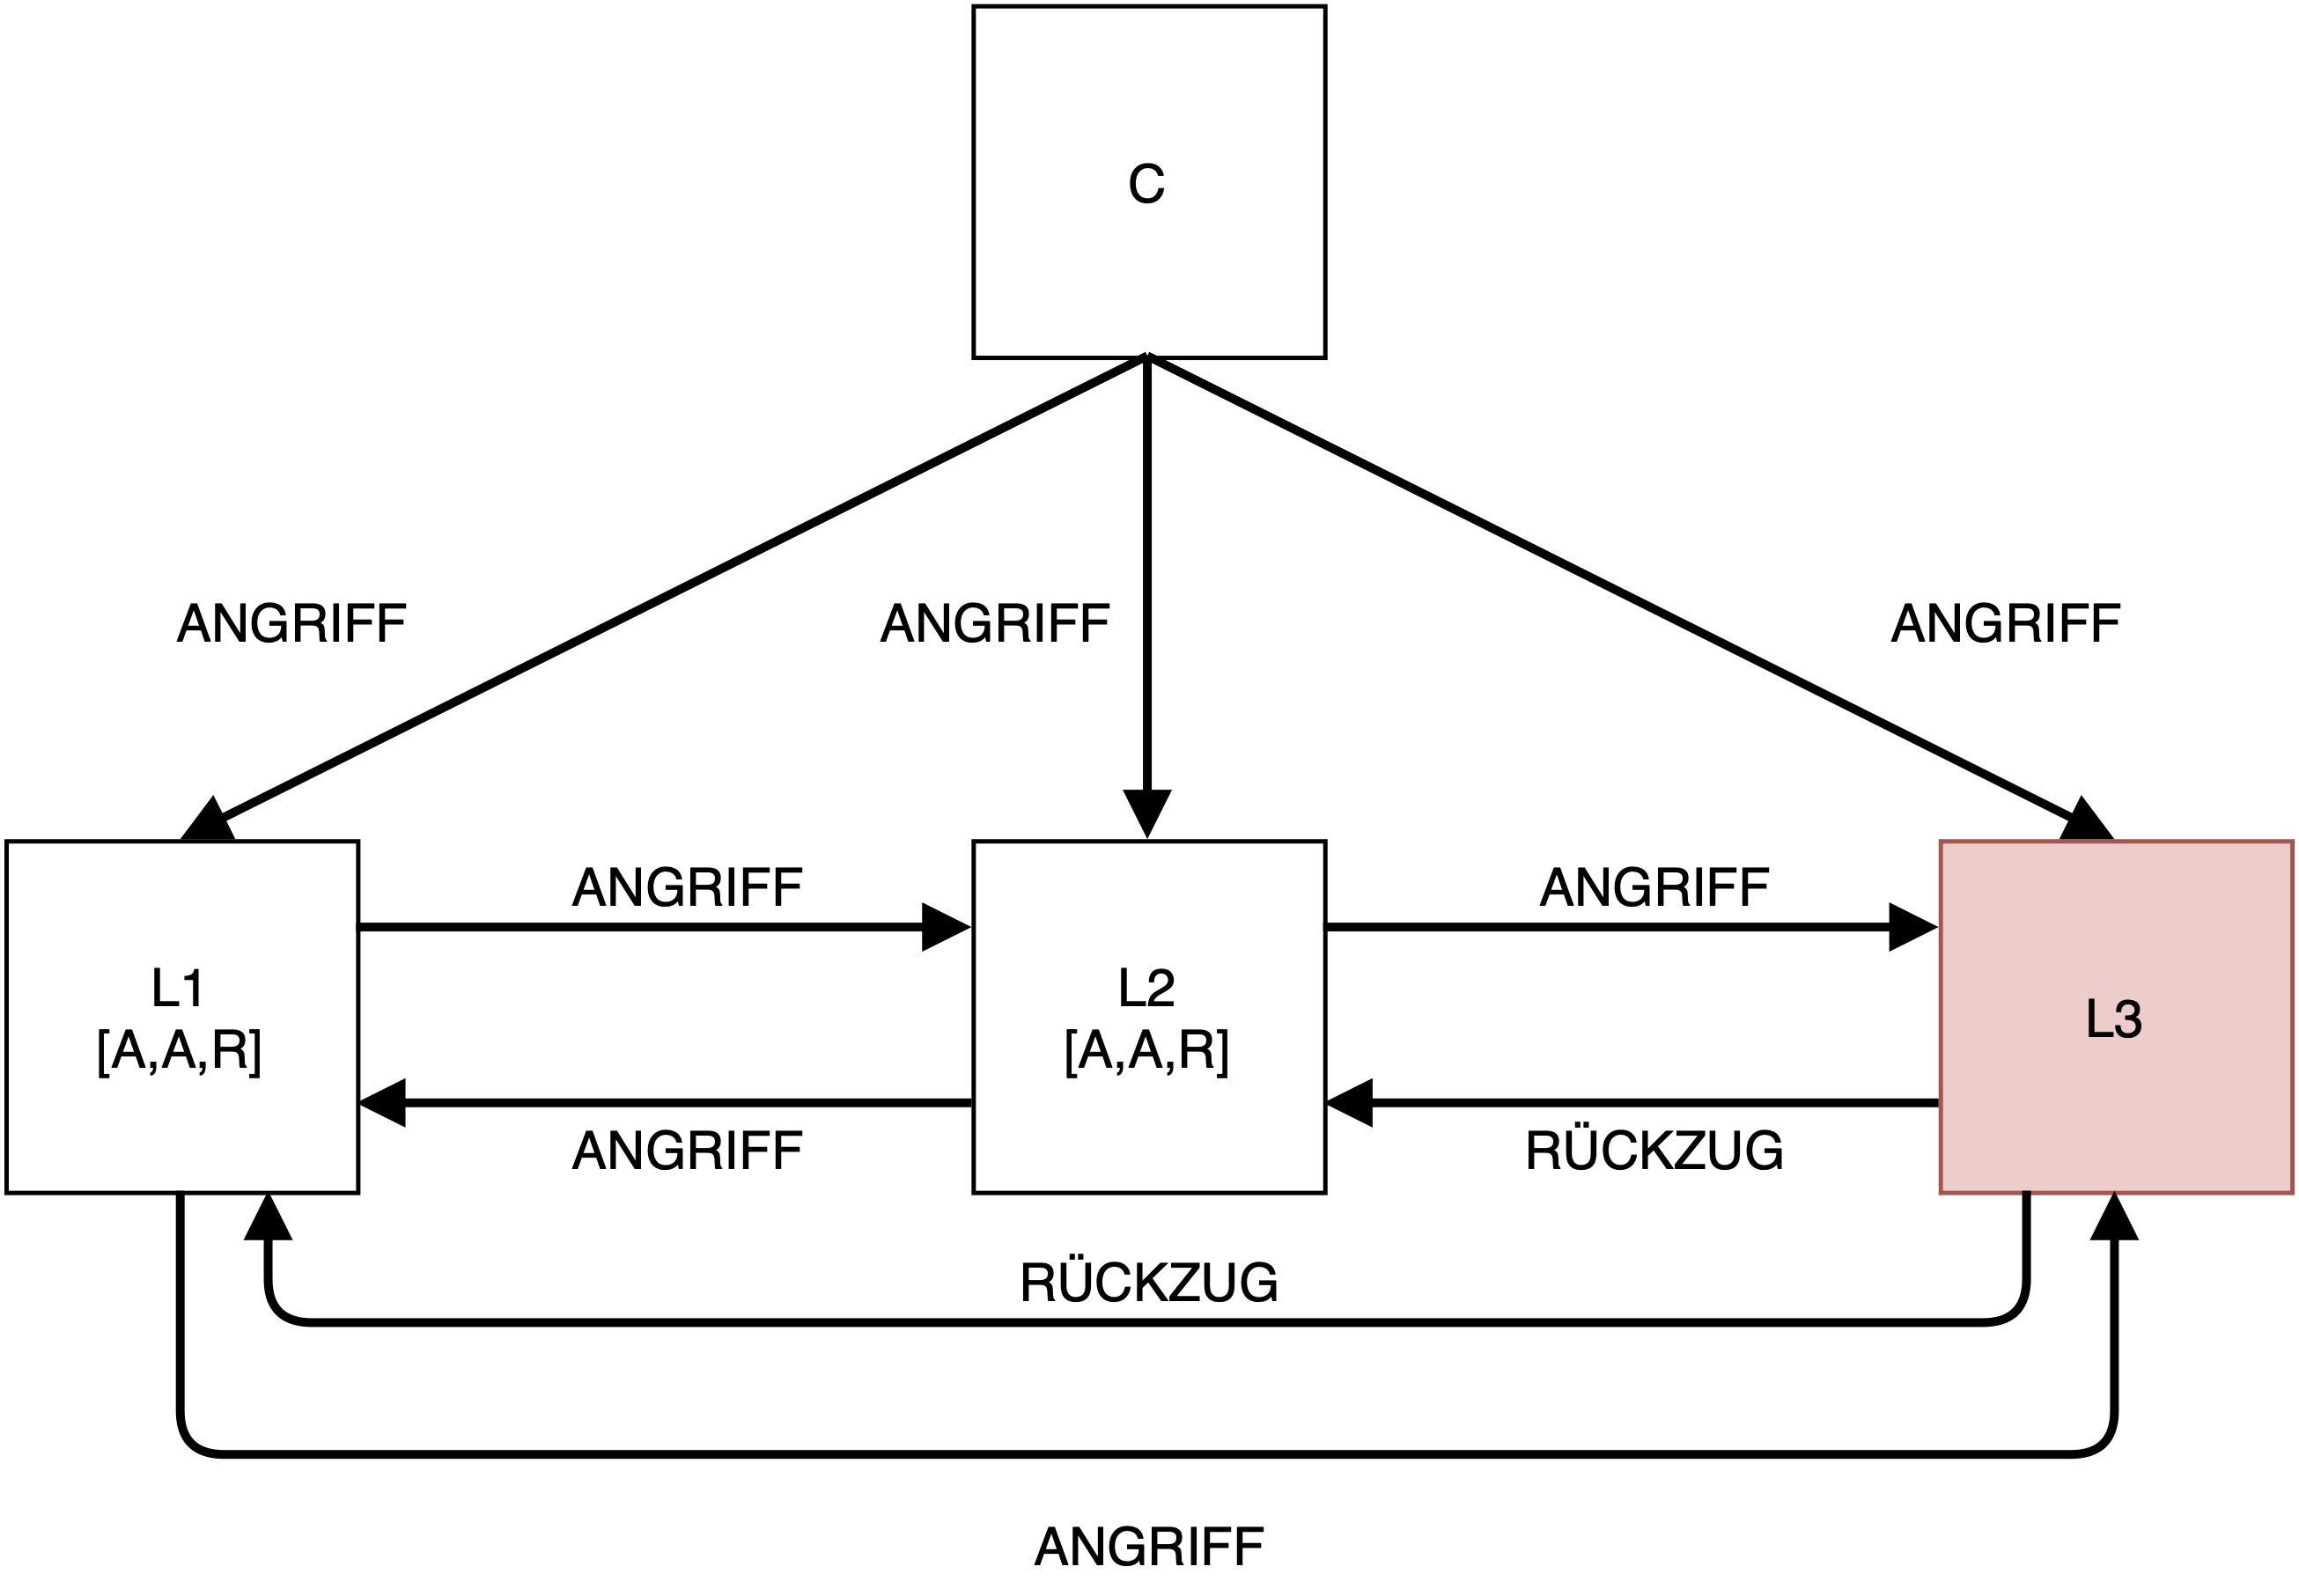
\includegraphics[width=0.8\textwidth]{omalgo.png}
    \caption{Zeigt, dass durch das Hinzufügen eines vierten Generals ein byzantinischer Fehler erkennt werden kann.}
    \label{fig:omalgo}
\end{figure}

\medskip 

Desweiteren, wäre der Einsatz von signierten Nachrichten eine andere valide Lösung. 
Dadurch könnte im Beispiel der Abbildung \ref{fig:general1} festgestellt werden,
dass L2 die Nachricht verfälscht hätte. 

\newpage 

\section{Anleitung zum C++ Beispiel}

In diesem Abschnitt wird das in Abbildung \ref{fig:general1} und \ref{fig:general2} 
dargestellte Problem mithilfe einer C++ Anwendung demonstriert. 

\subsection{Ein Lieutenant ist der Verräter}

Um das in Abbildung \ref{fig:general1} dargestellte Problem 
mit der Anwendung zu demonstrieren, müssen die Programme 
\textit{commander} und \textit{lieutenent} wie folgend aufgerufen werden.

\medskip 

Zunächst muss das \textit{lieutenent}-Programm zweimal gestartet werden. 

\begin{center}
    \begin{verbatim}
    $ ./lieutenant -p 10000 -n 10001
    [2020-04-10 09:53:01.043] [info] Waiting for order...

    ...

    $ ./lieutenant -t -p 10001 -n 10000
    [2020-04-10 09:53:01.043] [info] Waiting for order...
    \end{verbatim}
\end{center}

Der Parameter \textit{-p} definiert den Port des Lieutenants und
\textit{-n} den des benachbarten Lieutenants. Um den Lieutnant als 
Verräter zu starten wird bei L2 das Flag \textit{-t} übergeben. 

\medskip 

In einem echten Netzwerk, z.B. bestehend aus einem Sensor würde, falls ein Threshold 
unter- oder überschritten wird, der Sensor, der diese Veränderung als erstes aufgenommen hat,
die Rolle des Commanders übernehmen. Um dieses Verhalten zu simulieren, wird das 
\textit{commander}-Programm ausgeführt. Dabei stellen die Parameter \textit{-1} und \textit{-2} die Ports
der Lieutenents L1 und L2 dar. 

\begin{center}
    \begin{verbatim}
    $ ./commander -1 10000 -2 10001
    [2020-04-10 10:05:08.067] [info] Sending orders to L1 at :10000 and L2 at :10001
    [2020-04-10 10:05:08.068] [info] Sending order 'ANGRIFF' to L1
    [2020-04-10 10:05:08.068] [info] Sending order 'ANGRIFF' to L2
    \end{verbatim}
\end{center}

Wie in Abbildung \ref{fig:general1} dargestellt, sendet der loyale Commander den Befehl 
\textit{ANGRIFF} an beide Lieutenants.

\medskip 

Lieutenant L1 verhält sich dabei exact wie in Abbildung \ref{fig:general1} dargestellt. 
Die Problematik dabei ist, ob sich für den Befehl \textit{ANGRIFF} oder \textit{RÜCKZUG} 
entschieden wird, wie in \ref{sec:generals} beschrieben wurde.

\begin{center}
    \begin{verbatim}
    [2020-04-10 09:53:01.043] [info] Waiting for order...
    [2020-04-10 10:05:08.072] [info] Commander sent 'ANGRIFF' order
    [2020-04-10 10:05:08.072] [info] Send 'ANGRIFF' order to neighbour
    [2020-04-10 10:05:08.072] [info] Waiting for neigbour's order...
    [2020-04-10 10:05:08.075] [info] Neighbours order is 'RÜCKZUG'
    [2020-04-10 10:05:08.075] [info] Picking the majority of:
    [2020-04-10 10:05:08.075] [info] ANGRIFF
    [2020-04-10 10:05:08.075] [info] RÜCKZUG
    \end{verbatim}
\end{center}

\subsection{Der Commander ist der Verräter}

Das Starten der Programme ist analog zum vorherigen Abschnitt, jedoch mit dem Unterschied, dass das 
Flag \textit{-t} nun anstatt bei einem der Lieutenants, sondern beim Starten des Commanders 
übergeben werden muss.

\begin{center}
    \begin{verbatim}
    $ ./commander -1 10000 -2 10001 -t
    [2020-04-10 10:20:22.792] [info] Sending orders to L1 at :10000 and L2 at :10001
    [2020-04-10 10:20:22.793] [info] Commander is a traitor
    [2020-04-10 10:20:22.793] [info] Sending order 'ANGRIFF' to L1
    [2020-04-10 10:20:22.793] [info] Sending order 'RÜCKZUG' to L2
    \end{verbatim}
\end{center}

Wie hier beobachtet werden kann, sendet der Commander unterschiedliche Befehle zu L1 und L2. 

\medskip 

L1 beobachtet keine Veränderung. 

\begin{center}
    \begin{verbatim}
    $ ./commander -1 10000 -2 10001 -t
    [2020-04-10 10:20:17.134] [info] Waiting for order...
    [2020-04-10 10:20:22.796] [info] Commander sent 'ANGRIFF' order
    [2020-04-10 10:20:22.796] [info] Send 'ANGRIFF' order to neighbour
    [2020-04-10 10:20:22.796] [info] Waiting for neigbour's order...
    [2020-04-10 10:20:22.799] [info] Neighbours order is 'RÜCKZUG'
    [2020-04-10 10:20:22.799] [info] Picking the majority of:
    [2020-04-10 10:20:22.799] [info] ANGRIFF
    [2020-04-10 10:20:22.799] [info] RÜCKZUG
    \end{verbatim}
\end{center}

\newpage

\printbibliography

\end{document}